% automatically generated document using lt2circuiTikz
\documentclass[tikz,margin={2pt 2pt 2pt 2pt}]{standalone}
\usepackage[compatibility,siunitx,  americanvoltages, americancurrents, europeanresistors, europeaninductors, americanports,%
  straightlabels, fetbodydiode, straightvoltages]{circuitikz}
\usepackage{tikz,amsmath, amssymb,bm,color,pgfkeys,siunitx,ifthen,ulem}
\usepackage{pgfplots}
\pgfplotsset{compat=1.14}
\usetikzlibrary{shapes,arrows}
%\usepackage{agaramondc}					% Adobe Garamond, custom shape
%\renewcommand{\shapedefault}{rtl} % rtl: roman tabular lining

\input{latex_ext}

\usetikzlibrary{backgrounds,calc,positioning}

\usetikzlibrary{circuits.ee.IEC}
\usetikzlibrary{arrows}


% sym32a style

\ctikzset{tripoles/mos style/arrows}
\ctikzset{
	/tikz/circuitikz/quadpoles/coupler/width=1,%1.3
	/tikz/circuitikz/quadpoles/coupler/height=0.952,%1.3
	/tikz/circuitikz/quadpoles/coupler2/width=1,%1.3
	/tikz/circuitikz/quadpoles/coupler2/height=0.952,%1.3
	/tikz/circuitikz/quadpoles/transformer/width=1.425,%1.5
	/tikz/circuitikz/quadpoles/transformer/height=1.425,%1.5
	/tikz/circuitikz/quadpoles/transformer core/width=1.425,%1.5
	/tikz/circuitikz/quadpoles/transformer core/height=1.425,%1.5
	/tikz/circuitikz/quadpoles/gyrator/width=1.425,%1.5
	/tikz/circuitikz/quadpoles/gyrator/height=1.425,%1.5
	%/tikz/circuitikz/monopoles/tlinestub/width=0.1875,%0.25 no effect!
	/tikz/circuitikz/tripoles/american and port/height=0.95,%.8
	/tikz/circuitikz/tripoles/american nand port/height=0.95,%.8
	/tikz/circuitikz/tripoles/american or port/height=0.95,%.8
	/tikz/circuitikz/tripoles/american nor port/height=0.95,%.8
	/tikz/circuitikz/tripoles/american xor port/height=0.95,%.8
	/tikz/circuitikz/tripoles/american xnor port/height=0.95,%.8
	/tikz/circuitikz/bipoles/tline/height=0.4,%0.3
%	/tikz/circuitikz/bipoles/tline/width=1.2,%0.8
	/tikz/circuitikz/bipoles/diode/height=0.375,%
	/tikz/circuitikz/bipoles/diode/width=0.375,%
	/tikz/circuitikz/bipoles/varcap/height=0.375,%
	/tikz/circuitikz/bipoles/varcap/width=0.375,%
	/tikz/circuitikz/tripoles/triac/height=1.05,%
	/tikz/circuitikz/tripoles/triac/width=0.952,%
	/tikz/circuitikz/tripoles/thyristor/height=1.05,%
	/tikz/circuitikz/tripoles/thyristor/width=0.952,%
	/tikz/circuitikz/tripoles/op amp/height=0.952,%
	/tikz/circuitikz/tripoles/op amp/width=1.2,%
	/tikz/circuitikz/tripoles/op amp/font=\footnotesize,
	/tikz/circuitikz/tripoles/gm amp/height=0.952,% 1.7
	/tikz/circuitikz/tripoles/gm amp/width=1.2,% 1.4
	%	/tikz/circuitikz/tripoles/gm amp/font=\footnotesize,
	/tikz/circuitikz/tripoles/plain amp/height=0.952,% 1.7
	/tikz/circuitikz/tripoles/plain amp/width=1.2,% 1.4
	/tikz/circuitikz/bipoles/resistor/voltage/straight label distance/.initial=.8,
	/tikz/circuitikz/bipoles/generic/voltage/straight label distance/.initial=.8,
	/tikz/circuitikz/bipoles/inductor/voltage/straight label distance/.initial=.8,
	/tikz/circuitikz/bipoles/fullgeneric/voltage/straight label distance/.initial=.8,
	/tikz/circuitikz/bipoles/capacitor/voltage/straight label distance/.initial=1.0,
	/tikz/circuitikz/bipoles/thickness=1.6,
}
\ctikzset{v/.append style={/tikz/european voltages}}

\definecolor{netlabelcolor}{rgb}{0, 0, 0.25}
\definecolor{lttotitextcolor}{rgb}{0, 0.4, 0.25}
\definecolor{lttotidrawcolor}{rgb}{0.6, 0.6, 0.6}
\definecolor{netcolor}{rgb}{0, 0, 0.5}

\pgfkeys{/lt2ti/netlabel/font/.initial= \small}
\pgfkeys{/lt2ti/text/font/.initial= \small}

\pgfkeys{/lt2ti/Net/.style= {netcolor}}
\tikzstyle{dashdotdotted}=[dash pattern=on 3pt off 2pt on \the\pgflinewidth off 2pt on \the\pgflinewidth off 2pt]

\pgfkeys{/lt2ti/VArrow/.style= {->,>=latex}}
\pgfkeys{/lt2ti/SArrow/.style= {->,>=angle 90}}

\begin{document}%
	%\centering%
		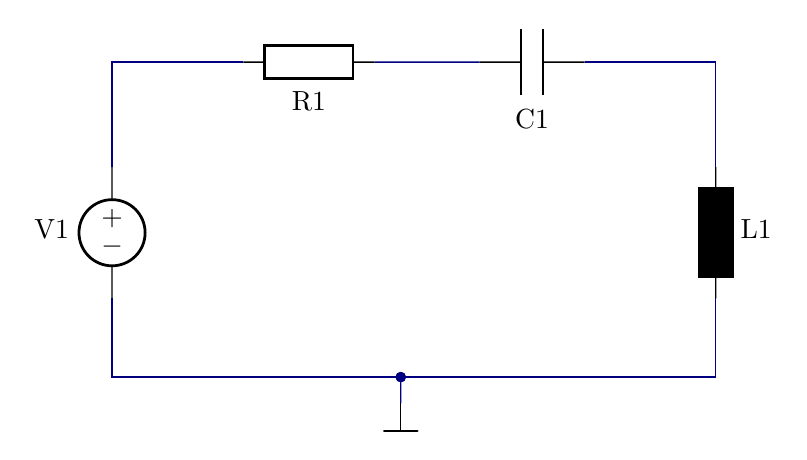
\begin{tikzpicture}[circuit ee IEC, scale=0.6666666667,line width=.5pt]% default: 0.4
	%\tikzstyle{every node}=[font=\small];%
	%\node [draw] at (0.0,0.0) {\pgfkeysvalueof{/tikz/circuitikz/tripoles/op amp/font}};
\draw [/lt2ti/Net](5.0,-2.5)to[*short,-, color=netcolor] (5.0,-2.5);% wire w3_w6 start
\draw [/lt2ti/Net](2.5,-4.5)to[*short,-, color=netcolor] (2.5,-4.5);% wire w3_w6 end
\draw [/lt2ti/Net](5.0,-2.5) --  (2.5,-2.5) -- (2.5,-4.5); % wire w3_w6 polyline 
\draw [/lt2ti/Net](9.5,-2.5)to[*short,-, color=netcolor] (7.5,-2.5);% wire w4
\draw [/lt2ti/Net](14.0,-4.5)to[*short,-, color=netcolor] (14.0,-4.5);% wire w5_w7 start
\draw [/lt2ti/Net](11.5,-2.5)to[*short,-, color=netcolor] (11.5,-2.5);% wire w5_w7 end
\draw [/lt2ti/Net](14.0,-4.5) --  (14.0,-2.5) -- (11.5,-2.5); % wire w5_w7 polyline 
\draw [/lt2ti/Net](8.0,-8.5)to[*short,*-, color=netcolor] (8.0,-8.5);% wire w8_w9 start
\draw [/lt2ti/Net](2.5,-7.0)to[*short,-, color=netcolor] (2.5,-7.0);% wire w8_w9 end
\draw [/lt2ti/Net](8.0,-8.5) --  (2.5,-8.5) -- (2.5,-7.0); % wire w8_w9 polyline 
\draw [/lt2ti/Net](14.0,-7.0)to[*short,-, color=netcolor] (14.0,-7.0);% wire w10_w11 start
\draw [/lt2ti/Net](8.0,-8.5)to[*short,-*, color=netcolor] (8.0,-8.5);% wire w10_w11 end
\draw [/lt2ti/Net](14.0,-7.0) --  (14.0,-8.5) -- (8.0,-8.5); % wire w10_w11 polyline 
\draw [/lt2ti/Net](8.0,-9.0)to[*short,-*, color=netcolor] (8.0,-8.5);% wire w12
 \draw (8.0, -9.0) node[rground, xscale=1, yscale=1, rotate=0, ] (undefined) {};%  (undefined)++(0.0,0.0) node {undefined }; % component "circuiTikz\gnd" "undefined" 
  \draw (2.5, -4.5) to[*V, l_=V1, a^=,, -, ] (2.5,-7.0){}; % component "voltage" "V1" 
  \draw (7.5, -2.5) to[*resistor, l^=R1, a_=, -, ] (5.0,-2.5){}; %\node [] at (8.0,-2.0) {x}; % component "res" "R1" 
  \draw (11.5, -2.5) to[*capacitor, l^=C1, a_=, -, ] (9.5,-2.5){}; % component "cap" "C1" 
  %\node [] at (11.5,-2.0) {x}; % component "cap" "C1" 
  \draw (14.0, -4.5) to[*inductor, l^=L1, a_=, - ] (14.0,-7.0){}; % component "ind" "L1" 
  %\node [] at (13.5,-4.0) {x}; % component "ind" "L1" 

	\end{tikzpicture}
\end{document}
